% ============================================================
%  Experiment 4 --- Interfacing FPGA to DIP Switch and Seven Segment
% ============================================================
\experimentheader{4}{Experiment 4}{Interfacing FPGA to DIP Switch and Seven Segment}{FPGA Lab}

\begin{objectives}
  \begin{enumerate}
    \item To use Verilog code as a design entry method in Altera Quartus II Software.
    \item To interface a DIP switch and a seven-segment display to the FPGA.
  \end{enumerate}
\end{objectives}

\begin{equipment}
  \begin{enumerate}
    \item Altera Quartus II software
          \begin{itemize}
            \item version 9/10/12 for Cyclone II
            \item version 9/10/12/latest for Cyclone IV
          \end{itemize}
    \item Altera DE2 board
    \item Function generator
  \end{enumerate}
\end{equipment}

\begin{introduction}
  Seven-segment displays are widely used to show numbers. The DE2 board provides eight seven-segment displays, 18 DIP switches, four push-button switches, and 16 LEDs. These components are hardwired on the board and are each assigned to specific FPGA pins --- refer to the DE2 user manual for the full pin map.
\end{introduction}

\begin{procedure}

  \textbf{Activity 1 --- 16-bit binary counter with frequency divider}\vspace{2pt}

  \textit{Objective: design a 16-bit binary counter driven through a frequency divider.}

  \begin{enumerate}
    \item Open Quartus II and write the frequency-divider module in Listing~\ref{lst:exp4-seven} (\texttt{seven}), which lowers the incoming clock frequency (Device family: Cyclone II (\texttt{EP2C35F672C6N}) or Cyclone IV (\texttt{EP4CE115F29C7N})).
    \item Create a reusable symbol for \texttt{seven}.
    \item Write the 4-bit counter module in Listing~\ref{lst:exp4-led} (\texttt{led}).
    \item Create a reusable symbol for \texttt{led}.
    \item Draw the schematic in Figure~\ref{fig:exp4-schematic}, connecting the \texttt{seven} block's most significant output bit \texttt{q[16]} to the clock input of the \texttt{led} block.
    \item Assign pin numbers as shown in Table~\ref{tab:exp4-pins} (refer to the DE2 user manual).
    \item Use a function generator to supply the clock signal, using 1\,MHz as the clock input.
    \item Determine the effective input frequency reaching the \texttt{led} module.
    \item Discuss your result based on the observed LED output display.
  \end{enumerate}

  \begin{codepanel}{seven.v --- frequency divider}{verilogstyle}
    \begin{lstlisting}
module seven(q, clk);
  output [15:0] q;
  input clk;
  reg [15:0] q;

  always @(posedge clk)
  begin
    q = (q + 1) % 65536;
  end
endmodule
\end{lstlisting}
  \end{codepanel}
  \vspace{-4pt}
  \listingcaption{lst:exp4-seven}{\texttt{seven.v} --- 16-bit frequency divider.}

  \begin{codepanel}{led.v --- 4-bit counter}{verilogstyle}
    \begin{lstlisting}
module led(x, clk);
  input clk;
  output [3:0] x;
  reg [3:0] x;

  always @(posedge clk)
  begin
    x = (x + 1) % 16;
  end
endmodule
\end{lstlisting}
  \end{codepanel}
  \vspace{-4pt}
  \listingcaption{lst:exp4-led}{\texttt{led.v} --- 4-bit binary counter.}

  \begin{boxedfigure}
    \centering
    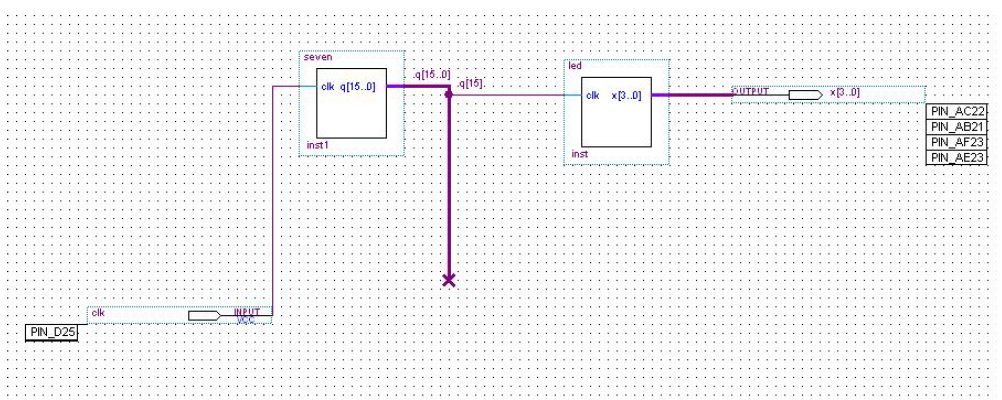
\includegraphics[width=0.85\linewidth]{figures/Exp4_Figure_1.png}
    \captionof{figure}{Schematic diagram for the 16-bit binary counter with frequency divider.}
    \label{fig:exp4-schematic}
  \end{boxedfigure}

  \needspace{4cm}
  \begin{boxedtable}
    \captionof{table}{Pin assignment for the 4-bit binary counter.}
    \label{tab:exp4-pins}
    {\renewcommand{\arraystretch}{1.5}
      \centering
      \begin{tabular}{cccc}
        \toprule
        \# & Node name & Direction & Pin location \\
        \midrule
        1  & clk       & Input     &              \\
        2  & X[3]      & Output    &              \\
        3  & X[2]      & Output    &              \\
        4  & X[1]      & Output    &              \\
        5  & X[0]      & Output    &              \\
        \bottomrule
      \end{tabular}
    }
  \end{boxedtable}
  \vspace*{1.5em}

  \textbf{Activity 2 --- 0--99 counter on seven-segment display}\vspace{2pt}

  \textit{Objectives: (1) design a counter that counts 0 to 99; (2) display the result on the seven-segment displays.}

  \begin{enumerate}
    \item Using a DIP switch as the trigger input, write Verilog code for a counter that counts from 0 to 99 once the switch is triggered.
    \item Decode and display the result (tens and units digits) on two seven-segment displays.
    \item Print and submit the Verilog code and simulation result.
  \end{enumerate}
  \vspace*{1em}

  \textbf{Activity 3 --- Running light}\vspace{2pt}

  \textit{Objective: design a running-light display on the Altera DE2 board.}

  \begin{enumerate}
    \item Using a DIP switch as the input, write Verilog code to implement a running-light (chasing LED) pattern.
    \item Use three DIP switches to select between three different running-light patterns.
    \item Print and submit the Verilog code and simulation result.
  \end{enumerate}

\end{procedure}
